\documentclass[border=1pt]{standalone}
\usepackage{mathptmx}  % Times text and math
\usepackage{circuitikz}
\usetikzlibrary{arrows.meta}
\ctikzset{bipoles/length=0.75cm, transistors/scale=0.9,
  inductors/coils=4, current/distance=.5, bipoles/diode/height=.32,
  bipoles/diode/width=.26}
\begin{document}
\fontsize{8}{9.6}\selectfont
% buck_charger: control diagram, 1 layout unit = 0.9622 cm (ieee-double)
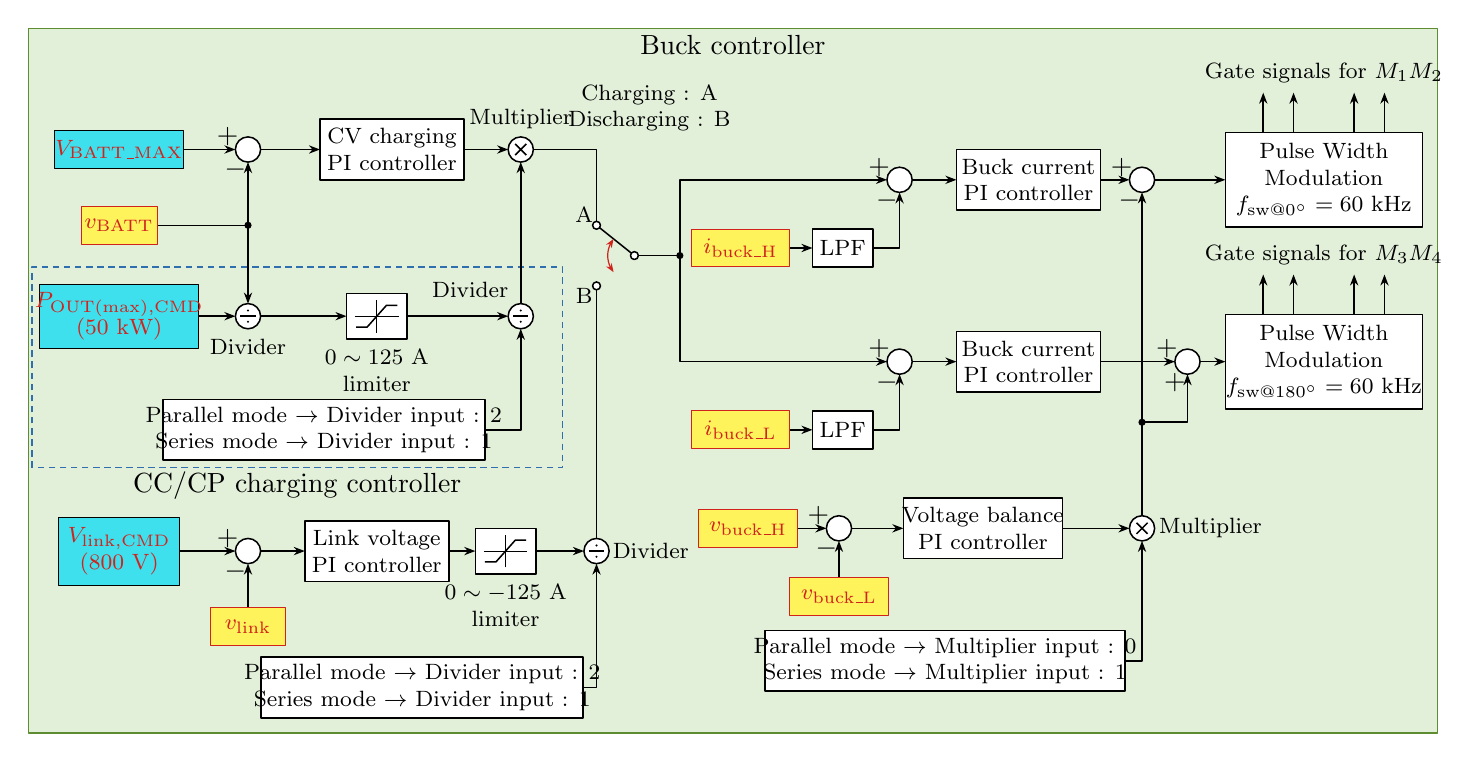
\begin{tikzpicture}[x=0.9622cm, y=0.9622cm, line width=0.55pt, line join=round]
% ---- regions (background) ----
\filldraw[fill={rgb,255:red,226;green,239;blue,217}, draw={rgb,255:red,94;green,140;blue,49}, line width=0.44pt] (-0.3,-4.7) rectangle (18.3,4.6);
\node[inner sep=0pt] at (9,4.3817) {Buck controller};
\draw[draw={rgb,255:red,47;green,111;blue,174}, line width=0.44pt, dash pattern=on 2.4pt off 1.6pt] (-0.25,-1.2) rectangle (6.75,1.45);
\node[inner sep=0pt] at (3.25,-1.439) {CC/CP charging controller};
% ---- links ----
\draw[-{Stealth[length=0.14cm]}] (1.75,3) -- (2.4337,3);
\draw[-{Stealth[length=0.14cm]}] (2.7663,3) -- (3.55,3);
\draw[-{Stealth[length=0.14cm]}] (5.45,3) -- (6.0337,3);
\draw[-{Stealth[length=0.14cm]}] (1.4,2) -- (2.6,2) -- (2.6,0.9663);
\draw[-{Stealth[length=0.14cm]}] (2.6,2) -- (2.6,2.8337);
\draw[-{Stealth[length=0.14cm]}] (1.95,0.8) -- (2.4337,0.8);
\draw[-{Stealth[length=0.14cm]}] (2.7663,0.8) -- (3.9,0.8);
\draw[-{Stealth[length=0.14cm]}] (4.7,0.8) -- (6.0337,0.8);
\draw[-{Stealth[length=0.14cm]}] (5.725,-0.7) -- (6.2,-0.7) -- (6.2,0.6337);
\draw[-{Stealth[length=0.14cm]}] (6.2,0.9663) -- (6.2,2.8337);
\draw (6.3663,3) -- (7.2,3) -- (7.2,2.052);
\draw[-{Stealth[length=0.14cm]}] (1.7,-2.3) -- (2.4337,-2.3);
\draw[-{Stealth[length=0.14cm]}] (2.6,-3.05) -- (2.6,-2.4663);
\draw[-{Stealth[length=0.14cm]}] (2.7663,-2.3) -- (3.35,-2.3);
\draw[-{Stealth[length=0.14cm]}] (5.25,-2.3) -- (5.6,-2.3);
\draw[-{Stealth[length=0.14cm]}] (6.4,-2.3) -- (7.0337,-2.3);
\draw[-{Stealth[length=0.14cm]}] (7.025,-4.1) -- (7.2,-4.1) -- (7.2,-2.4663);
\draw (7.2,-2.1337) -- (7.2,1.148);
\draw[-{Stealth[length=0.14cm]}] (7.752,1.6) -- (8.3,1.6) -- (8.3,2.6) -- (11.0337,2.6);
\draw[-{Stealth[length=0.14cm]}] (8.3,1.6) -- (8.3,0.2) -- (11.0337,0.2);
\draw[-{Stealth[length=0.14cm]}] (9.75,1.7) -- (10.05,1.7);
\draw[-{Stealth[length=0.14cm]}] (10.85,1.7) -- (11.2,1.7) -- (11.2,2.4337);
\draw[-{Stealth[length=0.14cm]}] (11.3663,2.6) -- (11.95,2.6);
\draw[-{Stealth[length=0.14cm]}] (13.85,2.6) -- (14.2337,2.6);
\draw[-{Stealth[length=0.14cm]}] (14.5663,2.6) -- (15.5,2.6);
\draw[-{Stealth[length=0.14cm]}] (9.75,-0.7) -- (10.05,-0.7);
\draw[-{Stealth[length=0.14cm]}] (10.85,-0.7) -- (11.2,-0.7) -- (11.2,0.0337);
\draw[-{Stealth[length=0.14cm]}] (11.3663,0.2) -- (11.95,0.2);
\draw[-{Stealth[length=0.14cm]}] (13.85,0.2) -- (14.8337,0.2);
\draw[-{Stealth[length=0.14cm]}] (15.1663,0.2) -- (15.5,0.2);
\draw[-{Stealth[length=0.14cm]}] (9.85,-2) -- (10.2337,-2);
\draw[-{Stealth[length=0.14cm]}] (10.4,-2.65) -- (10.4,-2.1663);
\draw[-{Stealth[length=0.14cm]}] (10.5663,-2) -- (11.25,-2);
\draw[-{Stealth[length=0.14cm]}] (13.35,-2) -- (14.2337,-2);
\draw[-{Stealth[length=0.14cm]}] (14.175,-3.75) -- (14.4,-3.75) -- (14.4,-2.1663);
\draw[-{Stealth[length=0.14cm]}] (14.4,-1.8337) -- (14.4,2.4337);
\draw[-{Stealth[length=0.14cm]}] (14.4,-0.6) -- (15,-0.6) -- (15,0.0337);
\draw[-{Stealth[length=0.14cm]}] (16,3.225) -- (16,3.75);
\draw[-{Stealth[length=0.14cm]}] (16.4,3.225) -- (16.4,3.75);
\draw[-{Stealth[length=0.14cm]}] (17.2,3.225) -- (17.2,3.75);
\draw[-{Stealth[length=0.14cm]}] (17.6,3.225) -- (17.6,3.75);
\draw[-{Stealth[length=0.14cm]}] (16,0.825) -- (16,1.35);
\draw[-{Stealth[length=0.14cm]}] (16.4,0.825) -- (16.4,1.35);
\draw[-{Stealth[length=0.14cm]}] (17.2,0.825) -- (17.2,1.35);
\draw[-{Stealth[length=0.14cm]}] (17.6,0.825) -- (17.6,1.35);
% ---- branch dots ----
\fill (2.6,2) circle (1.3pt);
\fill (8.3,1.6) circle (1.3pt);
\fill (14.4,-0.6) circle (1.3pt);
% ---- vbmax (tag) ----
\filldraw[fill={rgb,255:red,63;green,224;blue,238}, draw={rgb,255:red,0;green,0;blue,0}, line width=0.33pt] (0.05,2.75) rectangle (1.75,3.25);
% ---- sv (sum) ----
\draw[fill=white] (2.6,3) circle (0.16cm);
% ---- cvpi (block) ----
\draw[fill=white] (3.55,2.6) rectangle (5.45,3.4);
% ---- mx (mul) ----
\draw[fill=white] (6.2,3) circle (0.16cm);
\draw (6.2,3) ++(-0.0701cm,-0.0701cm) -- ++(0.1403cm,0.1403cm) (6.2,3) ++(-0.0701cm,0.0701cm) -- ++(0.1403cm,-0.1403cm);
% ---- vb (tag) ----
\filldraw[fill={rgb,255:red,255;green,243;blue,92}, draw={rgb,255:red,208;green,35;blue,28}, line width=0.33pt] (0.4,1.75) rectangle (1.4,2.25);
% ---- pout (tag) ----
\filldraw[fill={rgb,255:red,63;green,224;blue,238}, draw={rgb,255:red,0;green,0;blue,0}, line width=0.33pt] (-0.15,0.375) rectangle (1.95,1.225);
% ---- dv1 (div) ----
\draw[fill=white] (2.6,0.8) circle (0.16cm);
\draw (2.6,0.8) ++(-0.096cm,0) -- ++(0.192cm,0);
\fill (2.6,0.8) ++(0,0.072cm) circle (0.0144cm) (2.6,0.8) ++(0,-0.072cm) circle (0.0144cm);
% ---- lim1 (limiter) ----
\draw[fill=white] (3.9,0.5) rectangle (4.7,1.1);
\draw[line width=0.275pt] (4.012,0.8) -- (4.588,0.8) (4.3,0.584) -- (4.3,1.016);
\draw (4.028,0.656) -- (4.172,0.656) -- (4.428,0.944) -- (4.572,0.944);
% ---- dv2 (div) ----
\draw[fill=white] (6.2,0.8) circle (0.16cm);
\draw (6.2,0.8) ++(-0.096cm,0) -- ++(0.192cm,0);
\fill (6.2,0.8) ++(0,0.072cm) circle (0.0144cm) (6.2,0.8) ++(0,-0.072cm) circle (0.0144cm);
% ---- mode2 (block) ----
\draw[fill=white] (1.475,-1.1) rectangle (5.725,-0.3);
% ---- vlref (tag) ----
\filldraw[fill={rgb,255:red,63;green,224;blue,238}, draw={rgb,255:red,0;green,0;blue,0}, line width=0.33pt] (0.1,-2.75) rectangle (1.7,-1.85);
% ---- sl (sum) ----
\draw[fill=white] (2.6,-2.3) circle (0.16cm);
% ---- vlink (tag) ----
\filldraw[fill={rgb,255:red,255;green,243;blue,92}, draw={rgb,255:red,208;green,35;blue,28}, line width=0.33pt] (2.1,-3.55) rectangle (3.1,-3.05);
% ---- lvpi (block) ----
\draw[fill=white] (3.35,-2.7) rectangle (5.25,-1.9);
% ---- lim2 (limiter) ----
\draw[fill=white] (5.6,-2.6) rectangle (6.4,-2);
\draw[line width=0.275pt] (5.712,-2.3) -- (6.288,-2.3) (6,-2.516) -- (6,-2.084);
\draw (5.728,-2.444) -- (5.872,-2.444) -- (6.128,-2.156) -- (6.272,-2.156);
% ---- dvl (div) ----
\draw[fill=white] (7.2,-2.3) circle (0.16cm);
\draw (7.2,-2.3) ++(-0.096cm,0) -- ++(0.192cm,0);
\fill (7.2,-2.3) ++(0,0.072cm) circle (0.0144cm) (7.2,-2.3) ++(0,-0.072cm) circle (0.0144cm);
% ---- mode1 (block) ----
\draw[fill=white] (2.775,-4.5) rectangle (7.025,-3.7);
% ---- sw (switch) ----
\draw (7.6594,1.6325) -- (7.2406,1.9675);
\draw[{Stealth[length=0.112cm]}-{Stealth[length=0.112cm]}, draw={rgb,255:red,208;green,35;blue,28}, line width=0.44pt] (7.7,1.6) ++(141.3402:0.3389cm) arc[start angle=141.3402, end angle=218.6598, radius=0.3389cm];
\draw[fill=white] (7.7,1.6) circle (0.05cm);
\draw[fill=white] (7.2,2) circle (0.05cm);
\draw[fill=white] (7.2,1.2) circle (0.05cm);
% ---- b1 (sum) ----
\draw[fill=white] (11.2,2.6) circle (0.16cm);
% ---- ibh (tag) ----
\filldraw[fill={rgb,255:red,255;green,243;blue,92}, draw={rgb,255:red,208;green,35;blue,28}, line width=0.33pt] (8.45,1.45) rectangle (9.75,1.95);
% ---- lpf1 (block) ----
\draw[fill=white] (10.05,1.45) rectangle (10.85,1.95);
% ---- bpi1 (block) ----
\draw[fill=white] (11.95,2.2) rectangle (13.85,3);
% ---- c1 (sum) ----
\draw[fill=white] (14.4,2.6) circle (0.16cm);
% ---- pwm1 (block) ----
\draw[fill=white] (15.5,1.975) rectangle (18.1,3.225);
% ---- b2 (sum) ----
\draw[fill=white] (11.2,0.2) circle (0.16cm);
% ---- ibl (tag) ----
\filldraw[fill={rgb,255:red,255;green,243;blue,92}, draw={rgb,255:red,208;green,35;blue,28}, line width=0.33pt] (8.45,-0.95) rectangle (9.75,-0.45);
% ---- lpf2 (block) ----
\draw[fill=white] (10.05,-0.95) rectangle (10.85,-0.45);
% ---- bpi2 (block) ----
\draw[fill=white] (11.95,-0.2) rectangle (13.85,0.6);
% ---- c2 (sum) ----
\draw[fill=white] (15,0.2) circle (0.16cm);
% ---- pwm2 (block) ----
\draw[fill=white] (15.5,-0.425) rectangle (18.1,0.825);
% ---- vbh (tag) ----
\filldraw[fill={rgb,255:red,255;green,243;blue,92}, draw={rgb,255:red,208;green,35;blue,28}, line width=0.33pt] (8.55,-2.25) rectangle (9.85,-1.75);
% ---- vbl (tag) ----
\filldraw[fill={rgb,255:red,255;green,243;blue,92}, draw={rgb,255:red,208;green,35;blue,28}, line width=0.33pt] (9.75,-3.15) rectangle (11.05,-2.65);
% ---- sb (sum) ----
\draw[fill=white] (10.4,-2) circle (0.16cm);
% ---- vbpi (block) ----
\draw[fill=white] (11.25,-2.4) rectangle (13.35,-1.6);
% ---- mvb (mul) ----
\draw[fill=white] (14.4,-2) circle (0.16cm);
\draw (14.4,-2) ++(-0.0701cm,-0.0701cm) -- ++(0.1403cm,0.1403cm) (14.4,-2) ++(-0.0701cm,0.0701cm) -- ++(0.1403cm,-0.1403cm);
% ---- mode3 (block) ----
\draw[fill=white] (9.425,-4.15) rectangle (14.175,-3.35);
% ---- signs ----
\node[inner sep=0pt] at (2.3298,3.1663) {$+$};
\node[inner sep=0pt] at (2.4337,2.7298) {$-$};
\node[inner sep=0pt] at (2.3298,-2.1337) {$+$};
\node[inner sep=0pt] at (2.4337,-2.5702) {$-$};
\node[inner sep=0pt] at (10.9298,2.7663) {$+$};
\node[inner sep=0pt] at (11.0337,2.3298) {$-$};
\node[inner sep=0pt] at (14.1298,2.7663) {$+$};
\node[inner sep=0pt] at (14.2337,2.3298) {$-$};
\node[inner sep=0pt] at (10.9298,0.3663) {$+$};
\node[inner sep=0pt] at (11.0337,-0.0702) {$-$};
\node[inner sep=0pt] at (14.7298,0.3663) {$+$};
\node[inner sep=0pt] at (14.8337,-0.0702) {$+$};
\node[inner sep=0pt] at (10.1298,-1.8337) {$+$};
\node[inner sep=0pt] at (10.2337,-2.2702) {$-$};
% ---- text ----
\node[inner sep=0pt, align=center, font=\fontsize{8}{9.6}\selectfont, text={rgb,255:red,208;green,35;blue,28}] at (0.9,3) {$V_{\mathrm{BATT\_MAX}}$};
\node[inner sep=0pt, align=center, font=\fontsize{8}{9.6}\selectfont] at (4.5,3) {CV charging\\PI controller};
\node[inner sep=0pt, align=center, font=\fontsize{8}{9.6}\selectfont] at (6.2,3.4053) {Multiplier};
\node[inner sep=0pt, align=center, font=\fontsize{8}{9.6}\selectfont, text={rgb,255:red,208;green,35;blue,28}] at (0.9,2) {$v_{\mathrm{BATT}}$};
\node[inner sep=0pt, align=center, font=\fontsize{8}{9.6}\selectfont, text={rgb,255:red,208;green,35;blue,28}] at (0.9,0.8) {$P_{\mathrm{OUT(max),CMD}}$\\(50 kW)};
\node[inner sep=0pt, align=center, font=\fontsize{8}{9.6}\selectfont] at (2.6,0.3947) {Divider};
\node[inner sep=0pt, align=center, font=\fontsize{8}{9.6}\selectfont] at (4.3,0.0856) {$0\sim125$ A\\limiter};
\node[inner sep=0pt, align=center, font=\fontsize{8}{9.6}\selectfont] at (3.6,-0.7) {Parallel mode $\rightarrow$ Divider input : 2\\Series mode $\rightarrow$ Divider input : 1};
\node[inner sep=0pt, align=center, font=\fontsize{8}{9.6}\selectfont, text={rgb,255:red,208;green,35;blue,28}] at (0.9,-2.3) {$V_{\mathrm{link,CMD}}$\\(800 V)};
\node[inner sep=0pt, align=center, font=\fontsize{8}{9.6}\selectfont, text={rgb,255:red,208;green,35;blue,28}] at (2.6,-3.3) {$v_{\mathrm{link}}$};
\node[inner sep=0pt, align=center, font=\fontsize{8}{9.6}\selectfont] at (4.3,-2.3) {Link voltage\\PI controller};
\node[inner sep=0pt, align=center, font=\fontsize{8}{9.6}\selectfont] at (6,-3.0144) {$0\sim -125$ A\\limiter};
\node[inner sep=0pt, align=center, font=\fontsize{8}{9.6}\selectfont] at (7.9171,-2.3) {Divider};
\node[inner sep=0pt, align=center, font=\fontsize{8}{9.6}\selectfont] at (4.9,-4.1) {Parallel mode $\rightarrow$ Divider input : 2\\Series mode $\rightarrow$ Divider input : 1};
\node[inner sep=0pt, align=center, font=\fontsize{8}{9.6}\selectfont] at (7.0377,2.1299) {A};
\node[inner sep=0pt, align=center, font=\fontsize{8}{9.6}\selectfont] at (7.0377,1.0701) {B};
\node[inner sep=0pt, align=center, font=\fontsize{8}{9.6}\selectfont, text={rgb,255:red,208;green,35;blue,28}] at (9.1,1.7) {$i_{\mathrm{buck\_H}}$};
\node[inner sep=0pt, align=center, font=\fontsize{8}{9.6}\selectfont] at (10.45,1.7) {LPF};
\node[inner sep=0pt, align=center, font=\fontsize{8}{9.6}\selectfont] at (12.9,2.6) {Buck current\\PI controller};
\node[inner sep=0pt, align=center, font=\fontsize{8}{9.6}\selectfont] at (16.8,2.6) {Pulse Width\\Modulation\\$f_{\mathrm{sw@0^\circ}}=60$ kHz};
\node[inner sep=0pt, align=center, font=\fontsize{8}{9.6}\selectfont, text={rgb,255:red,208;green,35;blue,28}] at (9.1,-0.7) {$i_{\mathrm{buck\_L}}$};
\node[inner sep=0pt, align=center, font=\fontsize{8}{9.6}\selectfont] at (10.45,-0.7) {LPF};
\node[inner sep=0pt, align=center, font=\fontsize{8}{9.6}\selectfont] at (12.9,0.2) {Buck current\\PI controller};
\node[inner sep=0pt, align=center, font=\fontsize{8}{9.6}\selectfont] at (16.8,0.2) {Pulse Width\\Modulation\\$f_{\mathrm{sw@180^\circ}}=60$ kHz};
\node[inner sep=0pt, align=center, font=\fontsize{8}{9.6}\selectfont, text={rgb,255:red,208;green,35;blue,28}] at (9.2,-2) {$v_{\mathrm{buck\_H}}$};
\node[inner sep=0pt, align=center, font=\fontsize{8}{9.6}\selectfont, text={rgb,255:red,208;green,35;blue,28}] at (10.4,-2.9) {$v_{\mathrm{buck\_L}}$};
\node[inner sep=0pt, align=center, font=\fontsize{8}{9.6}\selectfont] at (12.3,-2) {Voltage balance\\PI controller};
\node[inner sep=0pt, align=center, font=\fontsize{8}{9.6}\selectfont] at (15.3042,-2) {Multiplier};
\node[inner sep=0pt, align=center, font=\fontsize{8}{9.6}\selectfont] at (11.8,-3.75) {Parallel mode $\rightarrow$ Multiplier input : 0\\Series mode $\rightarrow$ Multiplier input : 1};
\node[inner sep=0pt, align=center, font=\fontsize{8}{9.6}\selectfont] at (7.9,3.55) {Charging : A\\Discharging : B};
\node[inner sep=0pt, align=center, font=\fontsize{8}{9.6}\selectfont] at (16.8,4.0071) {Gate signals for $M_{1}M_{2}$};
\node[inner sep=0pt, align=center, font=\fontsize{8}{9.6}\selectfont] at (16.8,1.6071) {Gate signals for $M_{3}M_{4}$};
\node[inner sep=0pt, align=center, font=\fontsize{8}{9.6}\selectfont] at (5.5323,1.15) {Divider};
\end{tikzpicture}
\end{document}
